% Project 2 - EECS 499
% Author: Shaun Howard (smh150@case.edu)
\documentclass[conference]{IEEEtran} \usepackage[T1]{fontenc} \usepackage[backend=biber, style=ieee]{biblatex}
\addbibresource{report.bib} \usepackage[final]{microtype}

% graphics
\ifCLASSINFOpdf \usepackage[pdftex]{graphicx} % declare the path(s) where your graphic files are
  \graphicspath{{images/}} % and their extensions so you won't have to specify these with
  % every instance of \includegraphics
  \DeclareGraphicsExtensions{.jpeg,.png} \else
\fi


\begin{document}

\title{Jacobian Pseudo-inverse RRT Path Planner with Randomized-IK Restarts for Baxter Dual Arm Manipulator}

\author{
 \IEEEauthorblockN{Shaun Howard}
 \IEEEauthorblockA{Electrical Engineering and Computer Science Department\\
                   Case Western Reserve University\\ 
                   Cleveland, Ohio 44106\\
                   Email: smh150@case.edu}
}

% make the title area
\maketitle

% As a general rule, do not put math, special symbols or citations
% in the abstract
\begin{abstract}
Within this paper a flexible solution to the path planning problem for dual-arm robots is presented. Several methods are implemented for path planning with the 
Jacobian transpose and pseudo-inverse, using various forms of gradient descent. The construction of an Randomly RRT is presented which plans with the Jacobian 
pseudo-inverse for goal-directed movement and randomly restarts with a randomly-selected Inverse Kinematics solution point near the goal to avoid getting stuck 
in local minima. Several variations on the algorithm are tested, including switching between the Jacobian transpose and pseudo-inverse to compare planning 
accuracy, efficiency, and speed between the two gradient descent methods. The test results for the four algorithm combinations are compared. The results have 
yielded the focus of the paper to be on the pseudo-inverse gradient descent method for motion planning with random IK restarts for the Baxter dual arm 
manipulator.
\end{abstract}

\section{Introduction} \label{Introduction}

The search for accurate and quick planning algorithms has grown in recent years with major breakthroughs in memory architecture, processing unit speed and 
parallel processing. Several planning methods exist that were slow and infeasible to do in real-time in the past. These algorithms can now be resurrected and 
reused successfully on modern hardware. The planner described in this paper is a versatile planner that has several options for planning. The first option is to 
use only the Jacobian Transpose for planning. The algorithm for the RRT-JT from <paper1> influenced the JT planner implemented in this paper.  While this 
method's computational time is small and plans are accurate, it's planning capabilities are somewhat limited. The Jacobian Pseudo-inverse (JPI) adds yet more 
versatility to the planner by itself. The JPI planner utilized in this paper was influenced by multiple sources, primarily <paper2>. This method was also found to be a bit slow in descending to the goal. A method was implemented to increase the speed of descent as described in <paper3>. The implementation of this method allowed the planner to have two more variations, including the JT with speedup and JPI with speedup. 

A test bed was built for testing these algorithms with the Gazebo simulator, Rviz, and the Microsoft Xbox Kinect for Point Cloud environment visualization. An 
obstacle avoidance collision checker was added to detect obstacles and plan in avoidance of them during RRT construction. While experimenting with RRT 
construction, the nodes were found quick enough to unravel from the normal RRT construction pattern. The pattern is to create the entire tree and prune nodes, 
then to execute the path. That type of planning assumes a static environment that does not change during RRT construction. The planner framework presented in 
this paper updates obstacles upon each available update in an asynchronous fashion. This functionality is provided by creating a new ROS node that solely updates 
Kinect obstacle clouds for the robot to subscribe to with a ROS subscriber.

The Baxter robot has two 7 degree of freedom (DOF) arms. A multi-threaded extension was added to the planner to plan for both arms simultaneously and checking 
for obstacle collisions when validating solutions, while dynamically creating and executing RRT nodes on the robot. The obstacle collision checker filters 
each arm from its own obstacle cloud when possible. This allows each arm to plan in accordance for the other arm, to avoid collisions. Most of the experiments 
with the planner described in this paper isolate each arm from the other for testing accuracy and speed on complex goal poses. Poses ranging from easy to 
complex are tested and compared. The Jacobian PINV method paired with random IK restarts turned out to be the most effective and efficient method for motion 
planning with both arms as it is multi-threaded and modern computational power provides fast computation for the JPI.

The works related to the planner described in this paper are outlined in the next section. Following, the problem for dual-arm motion planning is established. After that, sensor measurements and capturing data with the Kinect setup are discussed. Later, the implementation is discussed along with experimentation and simulator set up. Second to last, experimentation results are analysed and compared. Lastly, the paper is concluded with the results of the experiments.

\begin{figure}
\label{pic1} 
\centering 
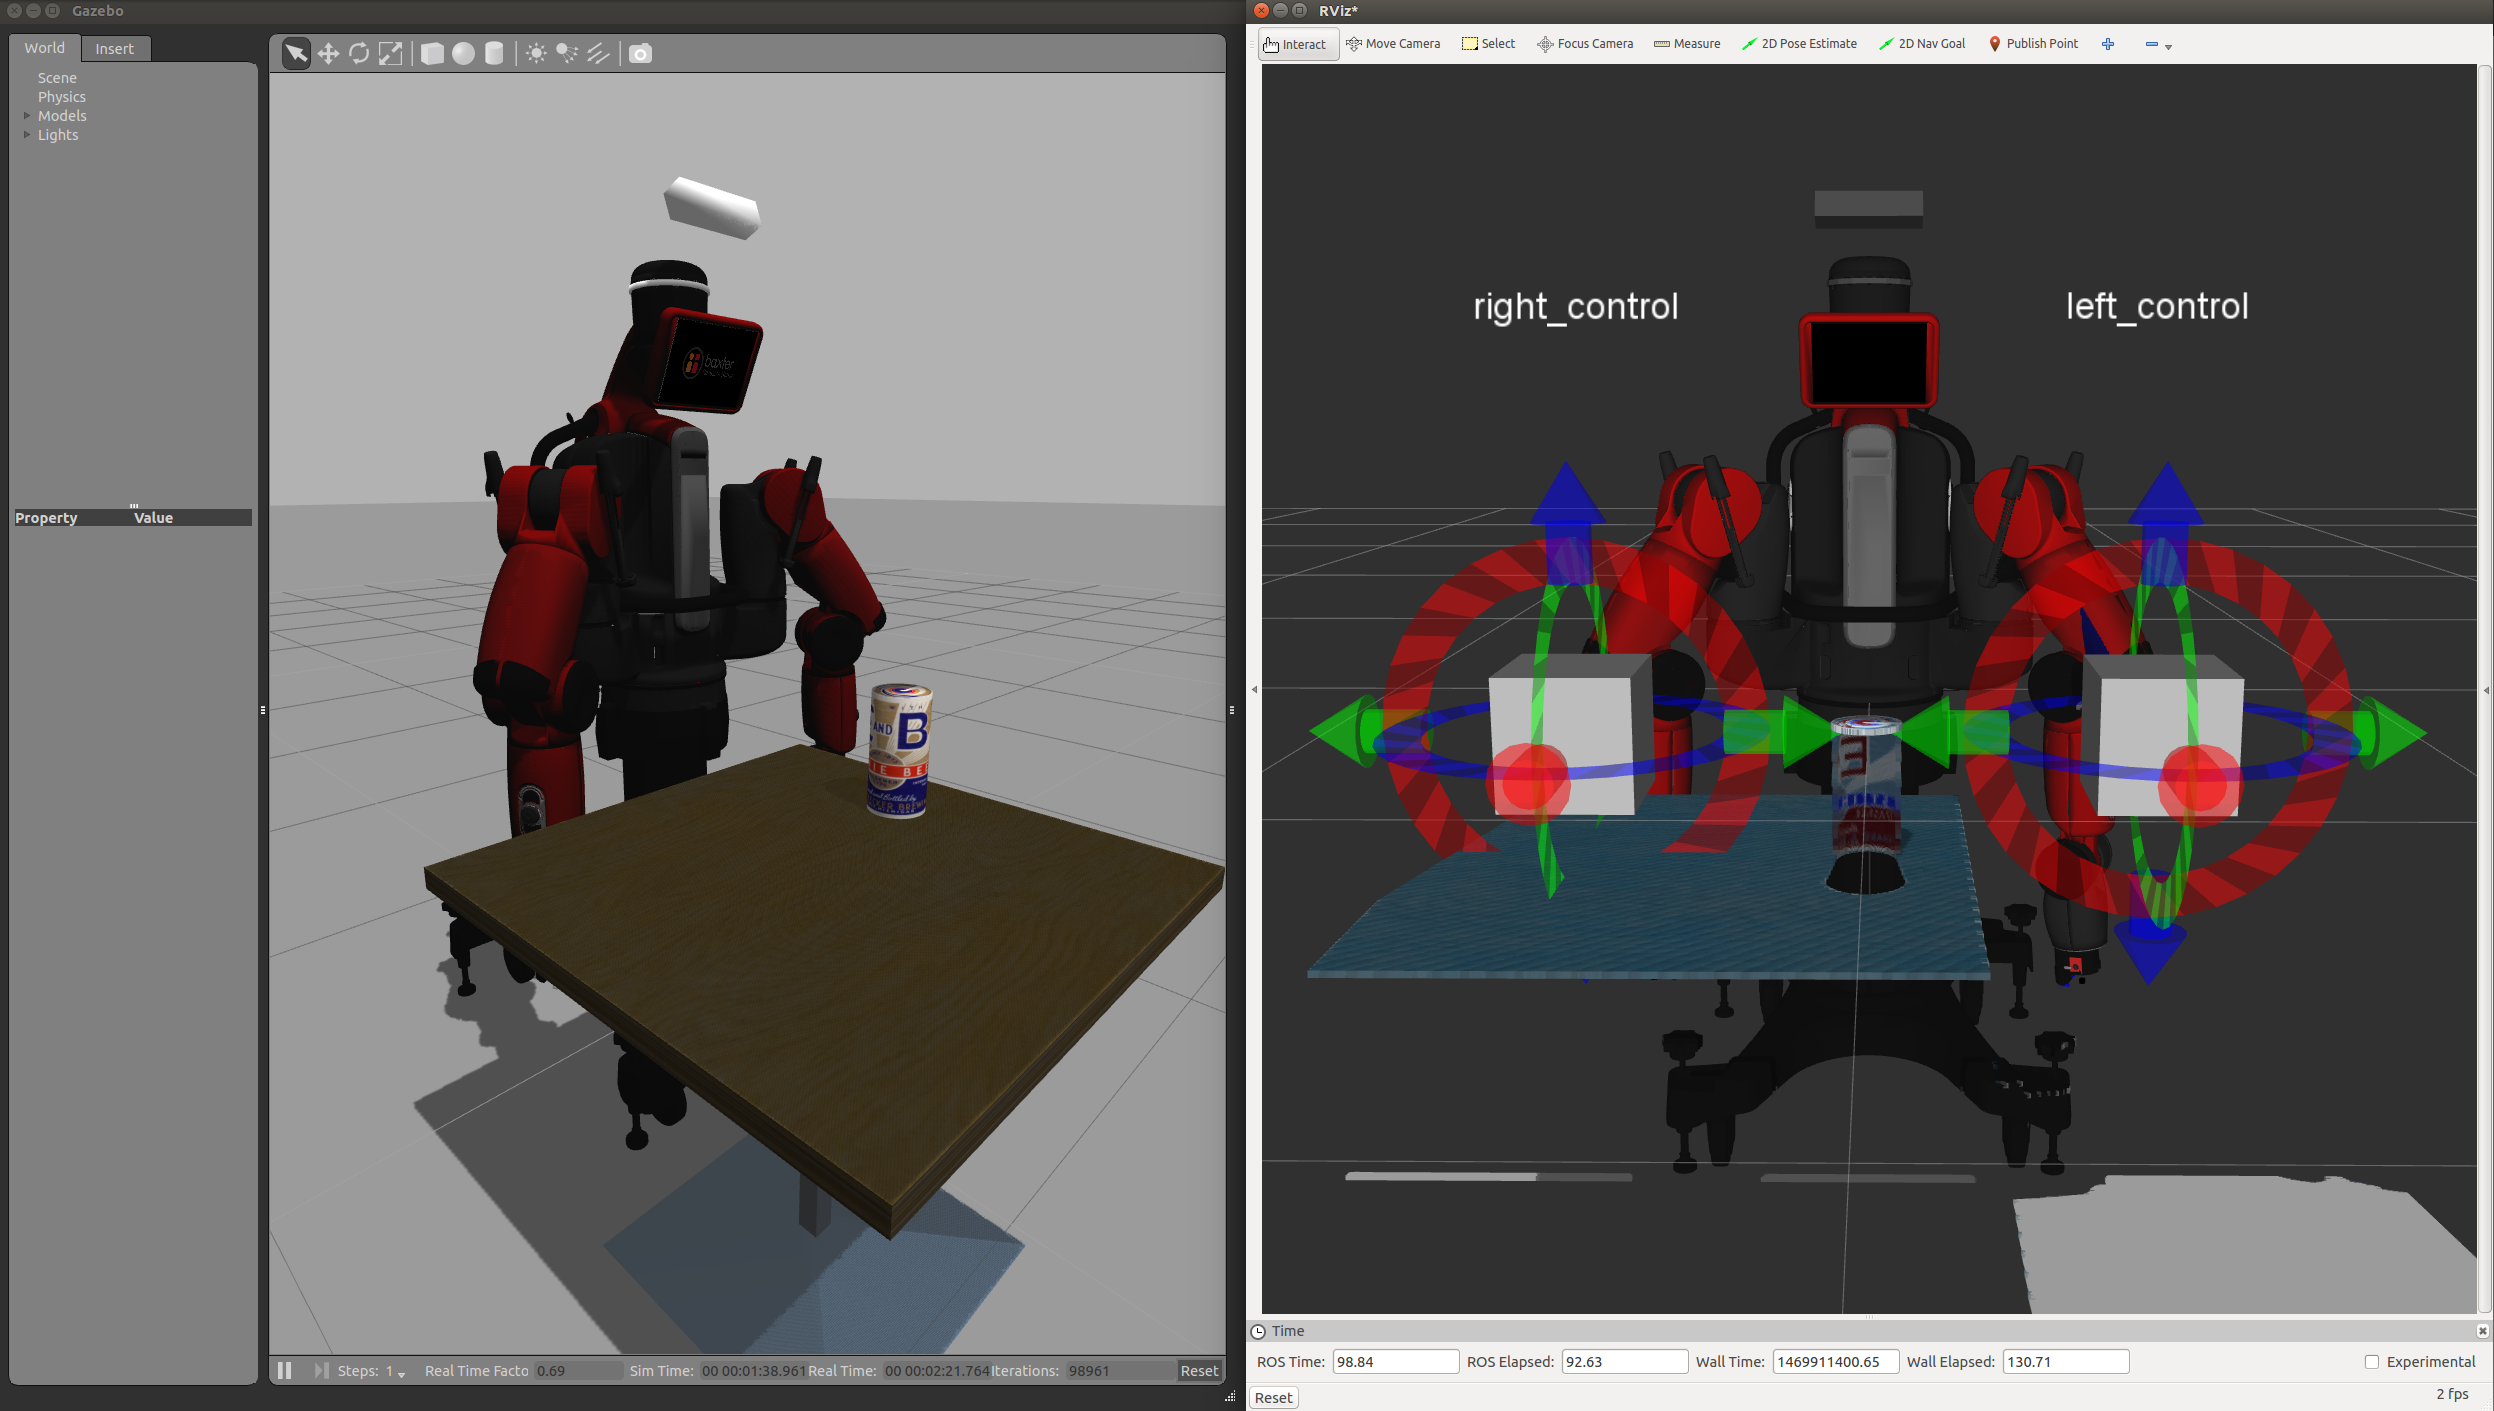
\includegraphics[width=0.49\textwidth]{sim1}
\caption{The Baxter simulator set-up with the Microsoft Xbox Kinect and some objects useful for obstacle detection in the scene.}
\end{figure}

\section{Related Work} \label{Related Work}

The first planner method used to implement the baseline planner was the RRT-JT, as implemented in <paper1>. This method was useful for getting the robot moving
and setting up a groundwork for accuracy and performance. The paper combines the idea of an RRT with the usage of a goal-directed modification to the typical
RRT algorithm, causing the end effector to approach the goal in a direction leading it closer to the goal than previous RRT methods. Another valuable aspect of 
this planner method is that it does not rely at all on IK solvers. The true pitch for this method is to be used in systems where IK solutions are hard or 
cost-ineffective to find.

The second planner method that the JPINV is based on is described in <paper2>. This paper focuses on diverse outlooks to the RRT-JT planner and make updates with the PINV and IK methods. They also feature dual-arm planning algorithms that plan for both arms simultaneously. Their paper outlines a modern framework of comparison for arm motion planning techniques that has provided this research with a sensible baseline for this planner using random PINV and IK solutions.

The third planner method is pioneered in the workspace goal region paper <paper3>. The paper utilizes concepts from <paper2> to holistically solve the obstacle
avoidance problem for motion planning. Workspace goal regions (WGR) are areas that the arm can operate in safely and efficiently. Outlying area is either 
inefficient or an impossible point to reach to say the least. The more advanced gradient descent method used to improve upon the first two planning methods is outlined in this paper. The method speeds up descent to local minima while the randomness is still at play in the planner because they apply the RRT-JT method.  

The fourth planner method was just discovered as an additional way to apply the JPINV method with the sped up gradient descent. The JT is switched with the 
JPINV and the planner improves in performance and accuracy. <paper2> inspired the use of the PINV in replacement of the transpose for this planning variation.

\section{Problem Formulation} \label{Problem Formulation}

Problem: need to plan quickly, on-the-go, with enough randomness not to get stuck as in stage fright in front of a crowd...

\section{Methodology} \label{Methodology}

Modifications were made to the concept of a Rapidly-
exploring Random Tree necessary to fuse several successful Jacobian-based techniques together to provide reliable redundant manipulator planning. This hybrid 
RRT planner uses the fusion of both the Jacobian-Transpose and Jacobian-Pseudoinverse-based methods for goal-directed path planning. For random path planning, a IK straight-line solver is used to 
sample solutions at random points within growing radii from the goal center until a goal is found or the maximum number of retires is met. The pairing of the 
hybrid RRT and random IK-based planner methods allow solutions to be found very quickly if possible, otherwise, the planner will get as close as possible over 
time or a minimum distance threshold is met. This method was found to perform better than the Jacobian-Transpose and IK-based approaches overall, although each 
method has upsides and downsides. Rarely, if ever, does the planner get noticeably stuck in local minima unless a goal is impossible for the end effector to 
reach. A Gazebo simulation paired with Rviz is used to examine custom implementations of the algorithms mentioned. A comparison is made between the methods used 
during experimentation which reveals that the hybrid RRT planner is quicker than the other planning methods while balancing constraints and generating a viable solution to almost any problem within reach of the given end effector in use.

\subsection{Sensor Measurements} \label{Sensor Measurements}

\subsection{Planner Implementation} \label{Planner Implementation}

\subsection{Gazebo Simulation} \label{Gazebo Simulation}

\section{Conclusion} \label{Conclusion} 

\subsection{Future Work}

\printbibliography
\end{document}